\section{Spektroskopie der Hyperfeinstruktur von Rubidium}
\subsection{Durchführung}
Bei der Messung des Hyperfein-Absorptionsspektrums befinden sich die beiden Linsen und
die Rubidiumzelle im Strahlengang.
Der Konstantanteil des Laserstroms, Modulationsamplitude und -frequenz
sind wie bei der Messung der Zeitabhängigkeit der Laserfrequenz (\autoref{sect:durchführung}).
Äußere Magnetfelder bleiben unkompensiert, weil die Zeeman-Aufspaltung der Hyperfeinstruktur im Erdmagnetfeld
mit der Linienbreite der Laserdiode nicht auflösbar ist.
Die Messung wird auf der steigenden und der fallenden Flanke der Modulationsspannung durchgeführt.


\subsection{Auswertung}
\subsubsection*{Frequenzkalibrierung}
\begin{figure}[H]
\begin{center}
  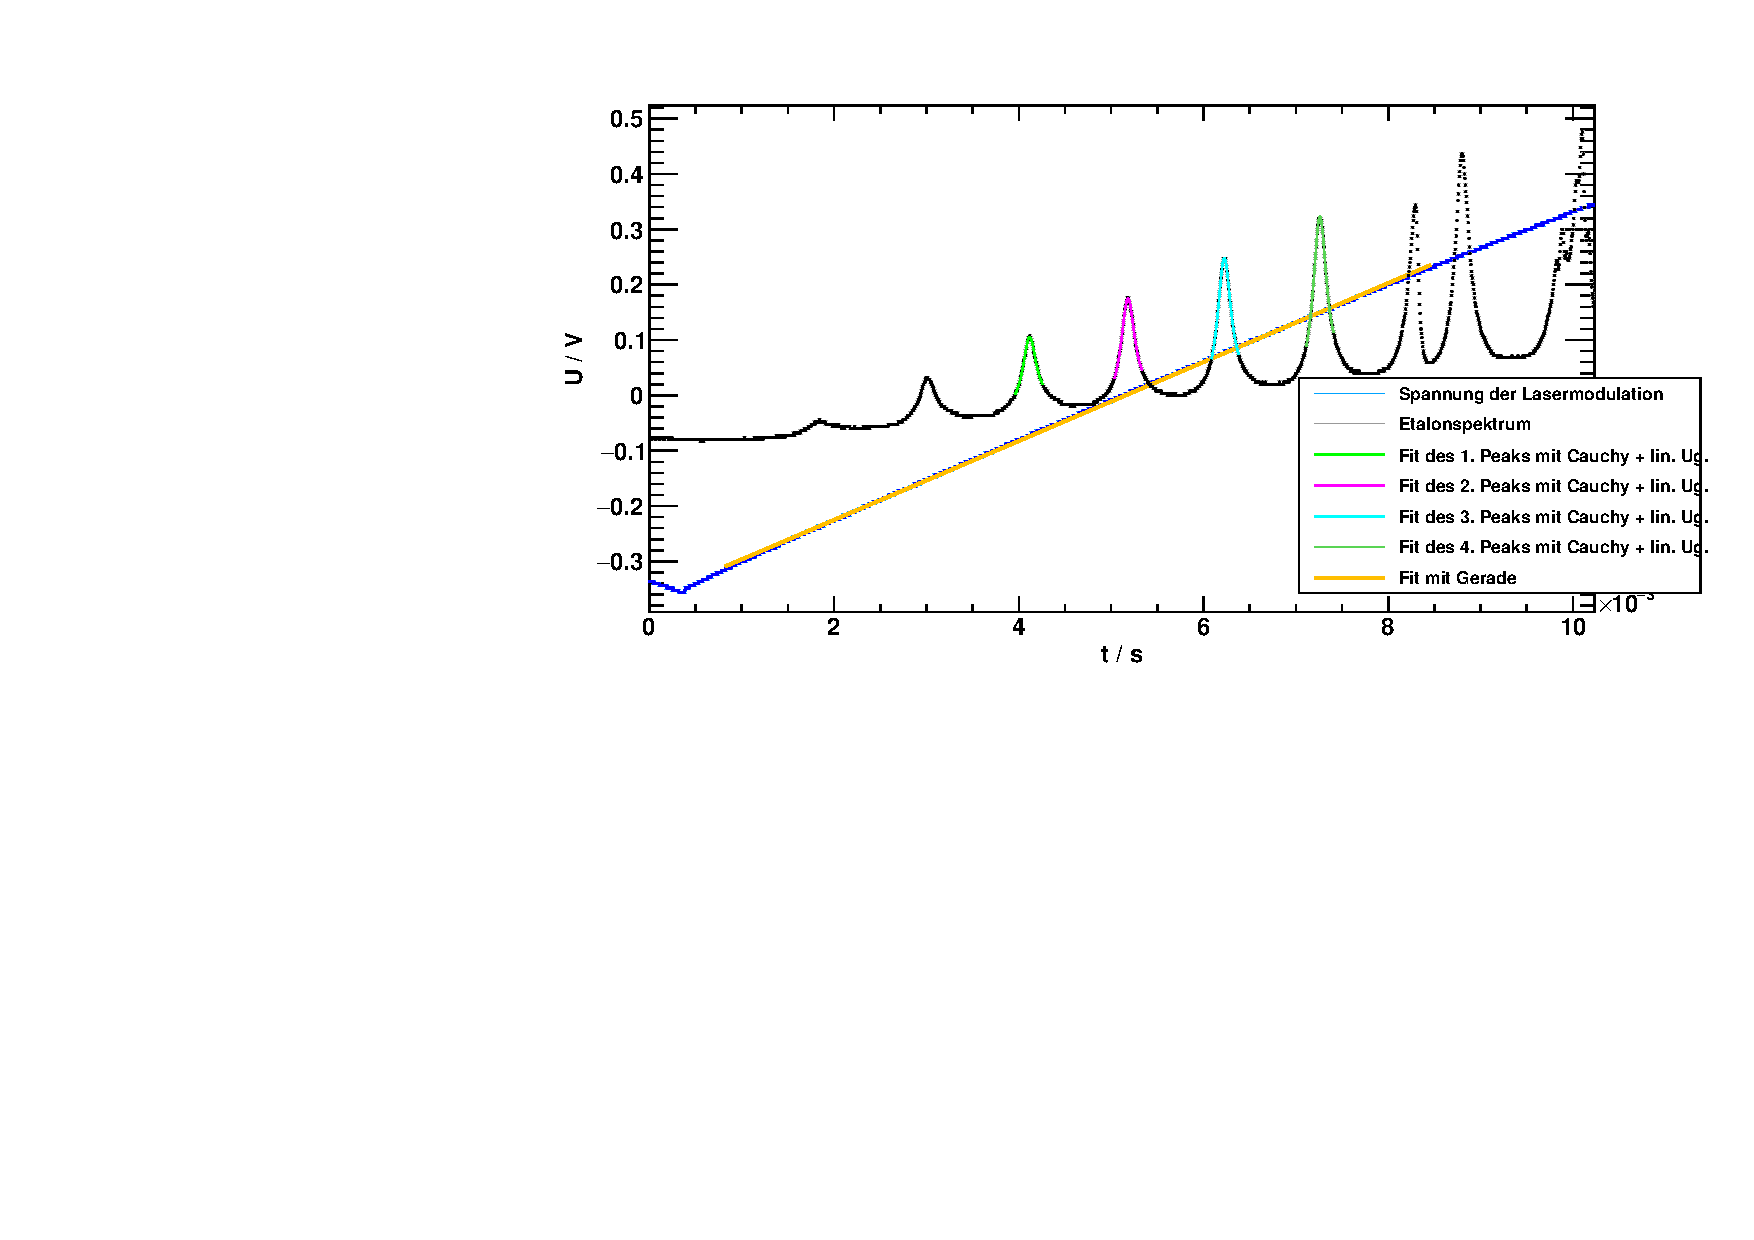
\includegraphics[width=\textwidth]{../img/part2/up-etalon_zoom_fit.pdf}
  \caption{caption.}
  \label{img:etalon:fit:up}
\end{center}
\end{figure}

\subsubsection*{Frequenzkalibrierung}
\begin{figure}[H]
\begin{center}
  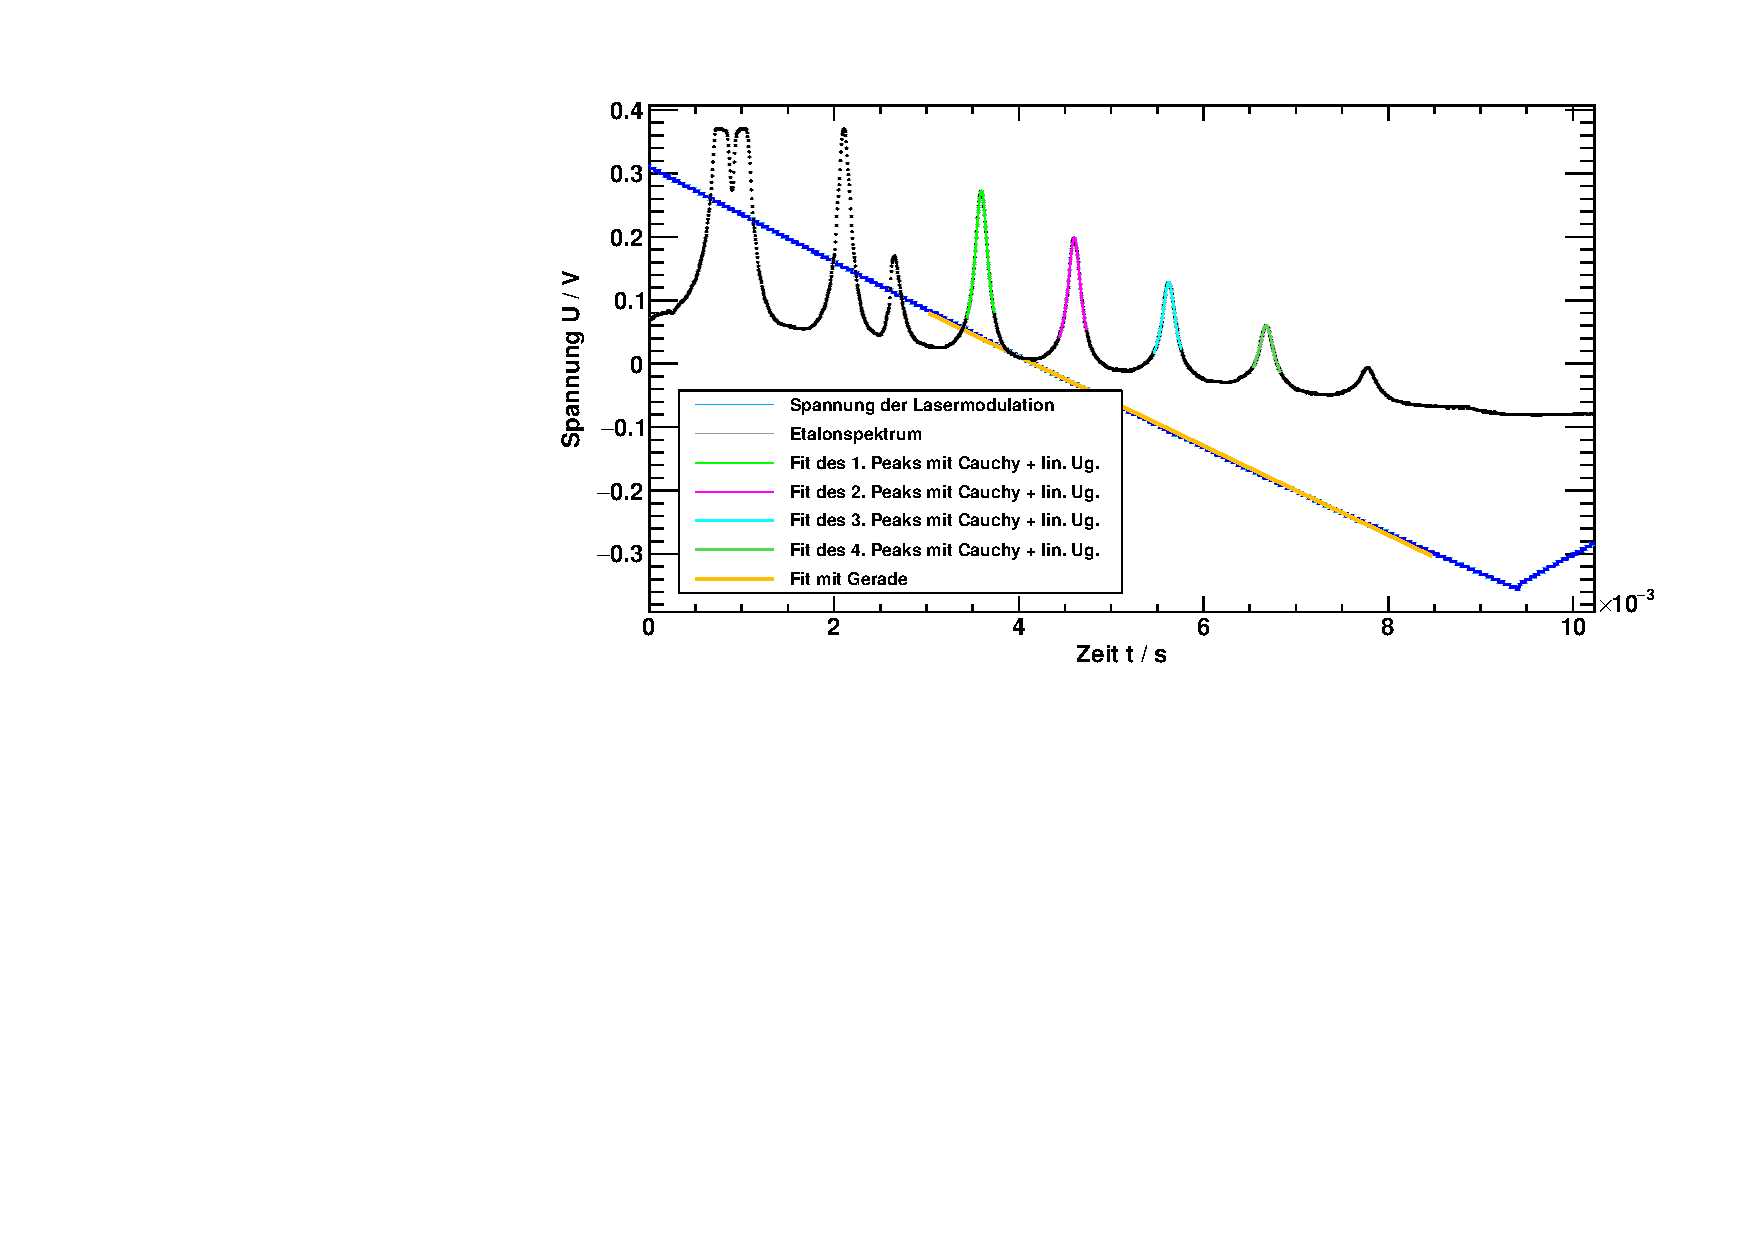
\includegraphics[width=\textwidth]{../img/part2/down-etalon_zoom_fit.pdf}
  \caption{caption.}
  \label{img:etalon:fit:down}
\end{center}
\end{figure}

\subsubsection*{Hyperfeinstruktur-Übergänge}
\subsubsection*{Berechnung des Spektrums}
\subsubsection*{Vergleich mit den Literaturwerten}
Gerade sollte Steigung 1 und Achsenabschnitt 0 Ghz haben